\documentclass{article}
\usepackage[utf8]{inputenc}
\usepackage{polski}
\usepackage[polish]{babel}
\usepackage{bbm}
\usepackage{graphicx}    
\usepackage{caption}
\usepackage{subcaption}
\usepackage{epstopdf}
\usepackage{amsmath}
\usepackage{amsthm}
\usepackage{hyperref}
\usepackage{url}
\usepackage{comment}
\newtheorem{defi}{Definicja}
\newtheorem{twr}{Twierdzenie}


\author{Kacper Kulczak 279079}
\date{Wrocław, \today}
\title{\textbf{Przybliżanie stałej matematycznej $e$ } \\ Sprawozdanie do zadania P.1.2}

\begin{document}
\maketitle
\section{Wstęp}

Wybrane przeze mnie zadanie polega na przybliżaniu stałej matematycznej $e$ (podstawy logarytmu naturalnego). Celem sprawozdania jest porównanie efektywności wybranych przeze mnie metod.
\\ \indent
 W \S 2 przedstawiono wyniki obliczeń przy korzystaniu z definicji liczby $e$. Metoda ta, została zasugerowana w treści zadania. W \S 3-4 sprawdzono inne sposoby na przybliżenie stałej $e$,  \S 5 natomiast, zawiera porównanie efektywność wybranych przeze mnie metod.
 \\ \indent
  Efektywność metod sprawdzano przez wyznaczenie ilość cyfr dokładnych do stałej (eu) w języku programowania Julia, za pomocą wyrażenia $-\log_{10}{|e-eu|}$ 
  \\ \indent
Wszystkie testy numeryczne przeprowadzone są przy użyciu programu \textbf{program.jl} w języku \textbf{Julia}, symulując tryb precyzji 256-bitowej. Plik \textbf{program.ipnyb} zawiera czytelną prezentacje uzyskanych wyników. 

\section{Definicja stałej $e$}

Jak wiadomo definicja stałej matematycznej $e$ to:

\begin{equation}\label{E:Def}
\lim_{n\to\infty} \left(1 + \frac{1}{n} \right) ^{n} =  e
\end{equation}

W programie \textbf{program.jl}, dołączonym do sprawozdania, zgodnie z treścią zadania obliczano stałą $e$ podstawiając pod $n$ kolejne potęgi ósemki. Algorytm wyliczał $1+\frac{1}{n}$, a następnie używał algorytmu szybkiego potęgowania . Wyniki przedstawiono w Tabeli \ref{Res,def}.

%TABLICA DEFINICJA
\begin{table}[h]
\centering
	\begin{tabular}{|c|c|} \hline
		n & Liczba cyfr dokładnych \\ \hline
		8 &  1\\
		$8^{2}$ &  2\\
		\vdots & \vdots \\
		$8^{29}$  &  26 \\
		$8^{30}$ &  27 \\
		\hline
	\end{tabular}
	\caption{Liczba cyfr dokładnych przy przybliżaniu stałej $e$ z definicji \eqref{E:Def}}
	\label{Res,def}
\end{table}

Po $8^{30}$ iteracji otrzymujemy jedynie $27$ cyfr dokładnych. Nie jest to wynik dobry, dlatego, też powinniśmy się przyjrzeć się innym metodom.
\\
\section{Ułamek łańcuchowy}
%CONTINUED FRACTION
Stałą matematyczną $e$ można  obliczyć również za pomocą prostego ułamka łańcuchowego Eulera \cite{CF}.

\begin{equation}\label{CF}
e = 2 + \frac{1}{1+\frac{1}{2+\frac{1}{1+\frac{1}{1+\frac{1}{4+\frac{1}{\vdots}}}}}}
\end{equation}

Ułamek \eqref{CF} można zapisać również w bardziej czytelnej notacji:  $e = [2;1;2;1;1;4;1;1;6;1;1;8...]$
W Tabeli \ref{res,cf} przedstawiony liczbę cyfr dokładnych wyliczoną dla kolejnych $n$. Algorytm, zastosowany w programie dołączonym do sprawozdania, w jednym kroku pętli oblicza $[1,1,2i]$, a następnie zmniejsza iterator o $2$. 

%TABLICA CONTIUNED FRACTION
\begin{table}[h] 
	\centering 
	\begin{tabular}{|c|c|}
		\hline
		n & Liczba cyfr dokładnych \\ \hline
		2 & 3 \\ 
		3 & 6 \\
		\vdots & \vdots \\
		20 & 66\\
		21 & 70\\
		\hline 
	\end{tabular}
	\caption{Liczba cyfr dokładnych, przy przybliżaniu stałej $e$, za pomocą prostego ułamka łańcuchowego Eulera}
	\label{res,cf}
\end{table}

Na podstawie wyników, możemy zauważyć, że ułamek łańcuchowy daje $70$ cyfr dokładnych przy $21$-ej iteracji. Możemy założyć, że algorytm daje nam około $3$ cyfry dokładne, na iteracje.

\section{Szeregi}

W matematyce występuje wiele szeregów zbieżnych do $e$. W tym sprawozdaniu wybrałem do testów dosłownie parę z nich: \cite{SZE}

%WZORY SZEREGI
\begin{equation}\label{szereg1}
e =  \sum_{i=0}^{\infty} \frac{1}{i!} 
\end{equation}
\begin{equation}\label{szereg2}
e =   \sum_{i=0}^{\infty}  \frac{3i+1}{\left(3i\right)!} 
\end{equation}
\begin{equation}\label{szereg3}
e = \left(\sum_{i=0}^{\infty}  \frac{4i+3}{2^{2i+1}\left(2i+1\right)!}\right)^{2}
\end{equation}

W Tabeli \ref{res,szeregi} przedstawiono, liczbę cyfr dokładnych, wyliczonych na podstawie dołączonego skryptu. Algorytm używał funkcji z biblioteki standardowej Julii "factorial(n)" do obliczania silni i sumował składniki od najmniejszego do największego.
\\
\begin{table}[h]
`	\centering
	\begin{tabular}{|c|c|c|c|}	\hline
		n & Szereg \eqref{szereg1} & Szereg \eqref{szereg2} & Szereg \eqref{szereg3} \\ \hline
		2 & 1& 4& 4 \\
		3 & 1& 7& 6 \\
		\vdots & \vdots & \vdots & \vdots \\
		17 & 16& 68& 52 \\
		18 & 17& 73& 56 \\ \hline
	\end{tabular}
	\caption{Liczba cyfr dokładnych przy przybliżeniu stałej e, za pomocą szeregów, dla odpowiedniej iteracji n}
	\label{res,szeregi}
\end{table}

Najlepsze wyniki uzyskano korzystając z szeregu \eqref{szereg2}, zyskując około $4$ cyfry dokładne na jedną iteracje. Natomiast szereg \eqref{szereg1}, zbiega powoli do $e$, zyskując około $1$ cyfrę dokładną na iteracje.

\section{Porównanie metod}

Na rysunku \ref{W1} przedstawiono w czytelny sposób wyniki doświadczeń zawartych w dołączonym do sprawozdania skrypcie.
\\\\\\\\\\\\\\\\\\\\
%WYKRES1
\begin{figure}[h]
\centering
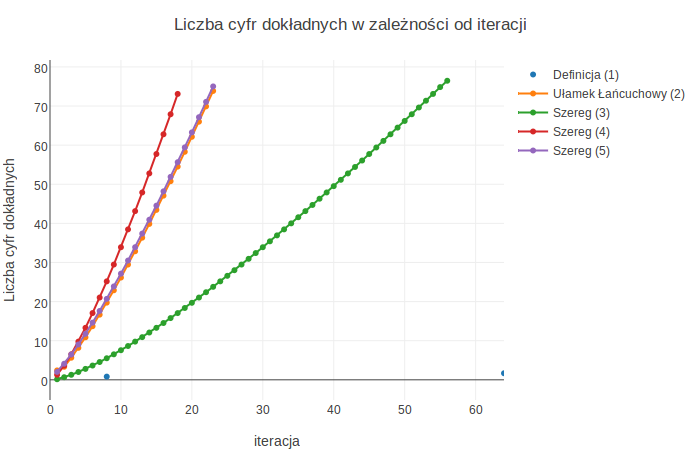
\includegraphics[width= 1 \textwidth]{wykres1.png}
\caption{Wykres porównujący liczbę cyfr dokładny w zależności od iteracji dla wzorów: \eqref{E:Def} \eqref{CF} \eqref{szereg1} \eqref{szereg2} \eqref{szereg3}}
\label{W1}
\end{figure}


Łatwo zauważyć, że najlepiej sprawdzającym się algorytmem jest szereg \eqref{szereg2}. Natomiast definicja \eqref{E:Def} nie nadaje się do przybliżania stałej $e$. 

Jednak jedna iteracja metody \eqref{E:Def} zawiera w sobie mniej operacji matematycznych niż iteracja metody \eqref{CF}
Dlatego, też zliczono ilość mnożeń oraz dzieleń, dla pojedynczej iteracji każdej z użytych metod. Dzięki temu uzyskano wiarygodniejsze porównanie.

\subsection{Ilość operacji mnożenie i dzielenia dla jednej iteracji}
	W poniższym wyliczeniu przedstawiono sposób obliczenia ilości mnożeń i dzieleń przy jednej iteracji. 
	\begin{enumerate}
		\item [\eqref{E:Def}] Na początku wykonujemy dzielenie $\frac{1}{n}$, a następnie przy użyciu, algorytmu szybkiego potęgowania wykonujemy $\log_{2}{n}$ mnożeń
		$$1+\log_{2}{n}$$
		
		\item [\eqref{CF}] W każdym wywołaniu pętli obliczamy $[1,1,2k]$. Są to $3$ dzielenia, co przy $n$ krokach daje nam :
		$$3n$$
		
		\item [\eqref{szereg1}]  Załóżmy, że zliczamy szereg pamiętając wyniki tymczasowe poprzedniego składnika. Wtedy wyliczenie $(n+1)!$ kosztuje nas tylko jedno mnożenie, bo $(n+1)! = n! * (n+1)$.
		\\ W takim wypadku przy pamiętanym $(n-1)!$, dla każdego składnika, potrzebujemy $1$ mnożenia i $1$ dzielenia, co daje nam:
		$$2n$$
		
		\item [\eqref{szereg2}] Zakładamy, że licznik zwiększany o $3$ i dzięki temu unikamy mnożenia w liczniku. Obliczenie silni, kolejnego składnika, kosztuje nas $3$ mnożenia. Trzeba wykonać jeszcze $1$ dzielenie. Powtarzamy to dla każdego składnika, więc otrzymujemy:
		$$4n$$
		
		\item[\eqref{szereg3}] Zakładamy, że nowy licznik to poprzedni powiększony o $4$ (unikamy mnożenia). Silnia kolejnego składnika kosztuje nas  $2$ mnożenia. W mianowniku wykonujemy jeszcze dodatkowe $2$ mnożenia ($4$ i potęga dwójki poprzedniego składnika). Do tego $1$ dzielenie. Powtarzamy dla każdego składnika oraz ostatnie podniesienie do kwadratu, więc otrzymujemy :
		$$5n + 1$$
	\end{enumerate}
%WYKRES 2
\begin{figure}[h]
	\centering
	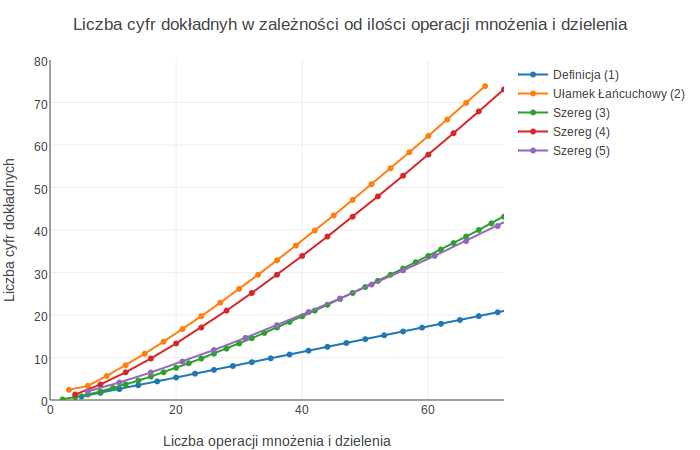
\includegraphics[width= 1 \textwidth]{wykres2.png}
	\caption{Wykres porównujący ilość wymaganych operacji mnożenia i dzielenia, do uzyskania określonej liczby cyfr dokładnych, przy użyciu następujących wzorów: \eqref{E:Def} \eqref{CF} \eqref{szereg1} \eqref{szereg2} \eqref{szereg3}}
	\label{W2}
\end{figure}

Z rysunku \ref{W2} wynika, że to ułamek łańcuchowy \eqref{CF} najefektywniej przybliża stałą matematyczną $e$. Ilość operacji, ukrytych w jednej iteracji, w szeregu \eqref{szereg3} sprawia, że wcale nie jest tak efektywny, jak wynikałoby z rysunku \ref{W1}. Warto też zauważyć, że mimo bardzo dobrej złożoności, definicja \eqref{E:Def} wciąż jest gorsza od każdej z wymienionych metod.

\section{Wnioski}


\indent
Zgodnie z podejrzeniami, w wyniku doświadczeń, pokazano niewielką przydatność definicji \eqref{E:Def} do przybliżania stałej matematycznej $e$.
\\ \indent
 Okazało się również że prosty ułamek łańcuchowy \eqref{CF} jest efektywniejszym sposobem na przybliżenie wartości $e$, od przedstawionych w sprawozdaniu szeregów. \\\indent
Sprawozdanie obrazuje również, że nieprecyzyjny sposób porównywania efektywności , może prowadzić do błędnych wniosków.


\begin{thebibliography}{9}
	\itemsep2pt
	\bibitem{CF} \url{http://mathworld.wolfram.com/EulersContinuedFraction.html}
	(ostatni dostęp do strony \today).
	
	\bibitem{SZE} \url{http://mathworld.wolfram.com/e.html}
	(ostatni dostęp do strony \today).
		
\end{thebibliography}

\end{document}
